\documentclass[sigconf]{acmart}

\usepackage{xspace,framed}
\usepackage{listings}

\setcopyright{acmcopyright}
\acmDOI{10.475/123_4}
\acmISBN{123-4567-24-567/08/06}
\acmConference[EMSOFT '17]{The ACM SIGBED International Conference on Embedded Software }{October 15--20, 2017}{Seoul, South Korea}
\acmYear{2017}
\copyrightyear{2017}
\acmPrice{15.00}


\newcommand\tool{{DSSynth Toolbox}\xspace}

\begin{document}

\title{DSSynth: An Automated Synthesis Tool for Physical Plants \\ Digital Controllers via MATLAB Toolbox}

\begin{abstract}
We present an automated approach implemented as a MATLAB Toolbox to synthesize stable and safe digital-control systems for physical plants represented as linear and time invariant models. The tool developed in the current paper is named as DSSynth (Digital-Systems Synthesis), which is a MATLAB Toolbox that synthesizes digital controllers w.r.t. the stability specification, considering finite word-length (FWL) effects for physical plants represented by transfer-function or state-space equations. DSSynth considers fixed-point numerical representation for the digital controller and dynamic input ranges for the closed-loop control system. Currently, there are two versions of the DSSynth toolbox: command-line and MATLAB application.
\end{abstract}

%
% The code below should be generated by the tool at
% http://dl.acm.org/ccs.cfm
% Please copy and paste the code instead of the example below. 
%
\begin{CCSXML}
<ccs2012>
<concept>
<concept_id>10010520.10010570</concept_id>
<concept_desc>Computer systems organization~Real-time systems</concept_desc>
<concept_significance>500</concept_significance>
</concept>
<concept>
<concept_id>10010520.10010553.10010562</concept_id>
<concept_desc>Computer systems organization~Embedded systems</concept_desc>
<concept_significance>300</concept_significance>
</concept>
<concept>
<concept_id>10011007.10010940.10010992.10010998.10003791</concept_id>
<concept_desc>Software and its engineering~Model checking</concept_desc>
<concept_significance>500</concept_significance>
</concept>
<concept>
<concept_id>10011007.10010940.10010992.10010998</concept_id>
<concept_desc>Software and its engineering~Formal methods</concept_desc>
<concept_significance>100</concept_significance>
</concept>
<concept>
<concept_id>10003752.10003790.10011192</concept_id>
<concept_desc>Theory of computation~Verification by model checking</concept_desc>
<concept_significance>300</concept_significance>
</concept>
</ccs2012>
\end{CCSXML}

\ccsdesc[500]{Computer systems organization~Real-time systems}
\ccsdesc[300]{Computer systems organization~Embedded systems}
\ccsdesc[500]{Software and its engineering~Model checking}
\ccsdesc[100]{Software and its engineering~Formal methods}
\ccsdesc[300]{Theory of computation~Verification by model checking}

\keywords{Formal Synthesis, Digital Controllers, MATLAB Toolbox, Fixed-point Arithmetic, Transfer-Function, State-Space, Digital Control Synthesis}

\maketitle

%---------------------------------------------------
\section{Introduction}
%---------------------------------------------------

%There are many application of embedded systems with low-cost devices that can perform non-trival tasks, such as UAV (Unmanned Aerial Vehicles) approach that could be used in various application (civil and millitary) that requires a reliable operation in order to avoid crashes and malfunctioning~\cite{williams2006human}. Synthesis of controllers for LTI (Linear Time Invariant) systems is broadly investigated, however the use of digital control architectures adds new challenges due to the effects of finite-precision arithmetic, time discretization, and quantization noise, which are typically introduced by Analogue-to-Digital (ADC) and Digital-to-Analogue (DAC) conversion~\cite{astrom1997computer}. 

%In addition, embedded systems present a lot of advantages, if compared with analog ones, such as more flexibility, scalability, adaptability, and lower implementation cost. However, embedded systems are expressed as digital-control systems which are vulnerable to finite word-length (FWL) effects~\cite{Guang2013, Istepanian2001}, that can cause several quantization problems, such as truncation or round-off errors.

Linear Time Invariant (LTI) systems are concepts that are used in many applications in order to support non-trivial tasks when applied in embedded systems. In addition, synthesis of controllers for LTI systems is richly studied by different researchers, however there are many challenges when digital-control systems theory is used due to the effects of finite-word length (FWL)~\cite{Guang2013, Istepanian2001}, time discretization, and quantization noise, which are typically introduced by Analogue-to-Digital (ADC) and Digital-to-Analogue (DAC) conversion, that can cause several quantization problems, such as truncation or round-off errors.~\cite{astrom1997computer}. 

Digital-control systems are computations that manipulate digital signals, in order to influence the behavior of a system~\cite{Ogata2001}; it can be mathematically expressed as difference equations, transfer functions, or state-space equations. In this particular work, the focus is on transfer-function and state-space representation. The following expression presents the general form of a digital-control system in transfer function format:
%
\begin{equation}
\small
\label{eq:transferfunction}
H(z)=\frac{B(z)}{A(z)}=\frac{b_{0}+b_{1}z^{-1}+...+b_{M}z^{-M}}{1+a_{1}z^{-1}+...+a_{N}z^{-N}},
\end{equation}
%
where $z^{-1}$ is called backward-shift operator, $A(z)$ and $B(z)$ are the denominator and numerator polynomials, respectively.

In state-space format, the digital-control system represents the behavior of a system through a state evolution equation $\dot{x}(n+1)$ and an instantaneous output equation $y(n)$, as follows:

\begin{equation}
\begin{split}
\dot{x}(n+1) &= A x(n) + B u(n)
\\
y(n) &= C x(n) + D u(n), 
\end{split}\label{eq:ss-example}
\end{equation}

%Recently, Bessa {\it et al.}~\cite{daes20161} has studied the stability of digital controllers considering implementation aspects, i.e., fixed-point arithmetic and the word length wich performs a model checking procedure based on satisfiability modulo theories (SMT) named as Digital-System Verifier (DSVerifier)~\cite{dsverifier}. While research on digital controller is well developed~\cite{astrom1997computer}, automated and sound control synthesis is challenging, particularly when the synthesis objective goes beyond classical stability. 

Recently, a new methodology to synthesize digital-control systems was designed, named as DSSynth (Digital-System Synthesizer)~\cite{abate2017, abatecav2017}, which is based on Counter-Example Guided Inductive Synthesis (CEGIS)~\cite{DBLP:conf/asplos/Solar-LezamaTBSS06} that are able to generate programs for highly non-trivial specifications with a very high degree of automation. Program synthesis engines use a specification as the starting point, and subsequently generate a sequence of candidate programs from a given template. The candidate programs are iteratively refined to eventually satisfy the specification. Modern synthesis engines combine automated testing, genetic algorithms, and SMT-based automated reasoning~\cite{DBLP:journals/corr/AlurFSS16a, DBLP:conf/lpar/DavidKL15}. Currently, Abate {\it et al.}~\cite{abate2017} synthesizes stable, software-implemented embedded controllers along with a model of a physical plant for transfer-function~\cite{abate2017}, and recently, also supports for state-space representation~\cite{abatecav2017}.

Notably, there are toolboxes in MATLAB with functions and scripts to facilitate the digital system design and implementation~\cite{matlab-toolbox}. In fact, there is a MATLAB Toolbox named as DSVerifier Toolbox~\cite{issta2017} that automatically detect specific errors related to digital system design ({\it e.g.}, stability) using symbolic model checking based on SAT and SMT solvers given the physical plant and the digital controller. However, there is no toolbox in MATLAB to perform the digital control synthesis based on Counter-Example Guided Inductive Synthesis (CEGIS)~\cite{DBLP:conf/asplos/Solar-LezamaTBSS06} considering FWL effects.

The present paper addresses this problem and presents a MATLAB toolbox for DSSynth~\cite{abate2017, abatecav2017} in the MATLAB's environment named as \tool. The main advantage regarding the use of a MATLAB toolbox lies on designing physical plants in MATLAB and then promptly synthesizes a stable digital controller. Additionally, when using the \tool, an engineer is able to design a digital system with MATLAB, through transfer-function or state-space representations, consider low-level systems parameters (implementation features and numerical format), and then gets a stable synthesized digital-controller.

%---------------------------------------------------
\section{Synthesizing Digital Controller with \tool}
%---------------------------------------------------

%---------------------------------------------------
\subsection{\tool Architecture}
%---------------------------------------------------

The proposed synthesization methodology for closed-loop digital systems is based on DSSynth~\cite{abate2017, abatecav2017} and it can be split into two main stages as follows: manual (user) and automated (DSSynth) procedures, as shown in Fig.~\ref{fig:synthesis-flow}. 

\begin{figure}[ht!]
\centering
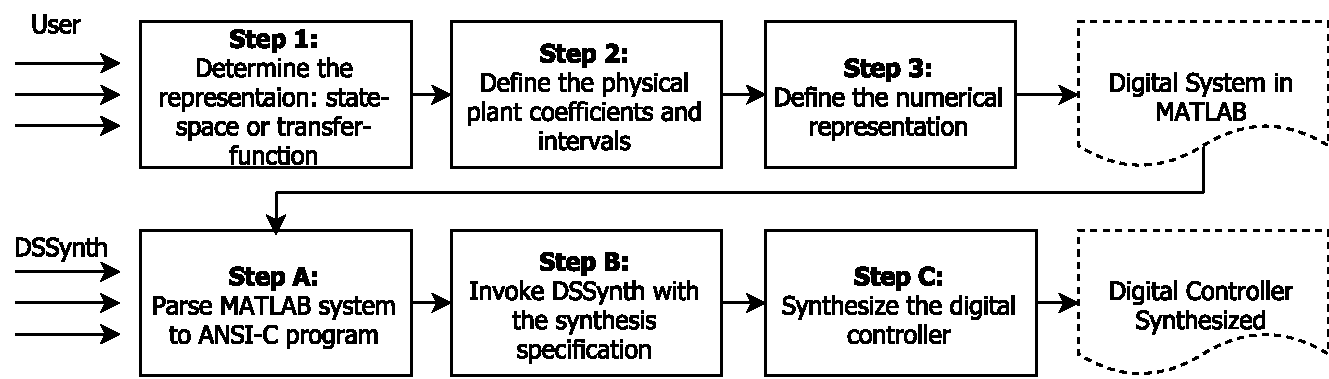
\includegraphics[width=0.45\textwidth]{synthesis-flow.pdf}
\caption{Digital-Control Synthesis Methodology.}
\label{fig:synthesis-flow}
\end{figure}

In step $1$, the digital-control representation is determined, and it could be in transfer-function or state-space equations. In step $2$, the physical plant with the coefficients must be designed according to equations (\ref{eq:transferfunction}) and (\ref{eq:ss-example}). And finally, in step $3$, the numerical representation with the digital-control implementation must be defined, {\it i.e.}, the FWL format that includes the number of bits in the integer and fractional parts and the dynamic range inputs. The result from the manual procedure is a digital-system implementation for the given physical plant in MATLAB. 

The synthesis process starts in step $A$, when the \tool gets the digital-system in MATLAB, and then translate it in a ANSI-C program, and then in step $B$, the DSSynth Tool is invoked. Finally, in step $C$, the digital controller is synthesized based on (CEGIS)~\cite{DBLP:conf/asplos/Solar-LezamaTBSS06}. The output generated in MATLAB is the digital controller synthesized, and it could be represented in transfer-function or state-space format. The synthesis is \emph{successful} when a digital controller is synthesized correctly, and the synthesis has status \emph{failed} when any parameter is defined incorrectly in previous steps, or there is no solution for the digital-system designed.
 
%---------------------------------------------------
\subsection{\tool Procedures}
%---------------------------------------------------

The \tool performs the following automated procedures in order to synthesize a digital controller:

\begin{enumerate}
\item \textbf{Setup}: obtain the plant, fixed-point format and dynamic input ranges, and translate them to a struct in MATLAB;
\item \textbf{Parse}: obtain the digital plant implementation, and then translate it to an ANSI-C file;
\item \textbf{Execute}: obtain the ANSI-C file from the previous step, call CBMC-CEGIS as back-end program synthesis tool, and then perform the automated synthesis;
\item \textbf{Extract}: obtain the .log that is generated after the synthesis phase and then check the synthesized digital-controller.
\item \textbf{Report}: obtain the digital-controller, translate it to a MATLAB system, and then show the result to the user.
\end{enumerate}

%---------------------------------------------------
\subsection{\tool Features}
%-----------------------------------------------

The \tool's features can be described as follows:

\begin{itemize}
\item \textbf{Representation}: the synthesis could be performed for digital-systems in transfer-function or state-space equations;
\item \textbf{Fixed-Point Arithmetic}: the digital controller is synthesized considering FWL effects, in fixed-point numeric representation;
\item \textbf{Interface}: the synthesis could be executed using the command-line version, and a GUI Application version. In addition, in the GUI Application, the user is able to plot the step response in order to reproduce the stability of the digital controller synthesized;
\end{itemize}
%---------------------------------------------------
\subsection{\tool Usage}
%---------------------------------------------------

%---------------------------------------------------
\subsubsection{Command Line Version}
%---------------------------------------------------

Users must provide a digital system described as a MATLAB system  using a \texttt{``tf''} (for transfer-function) or an \texttt{``ss''} (for state-space) command (cf. step $1$ of Fig.~\ref{fig:synthesis-flow}).

\tool is called via command line in MATLAB as \texttt{synthesize(plant, intBits, fracBits, maxRange, minRange)}, where \texttt{plant} is the physical plant in state-space or transfer-function representation, \texttt{intBits} is the integer part, \texttt{fracBits} is the fractional part, \texttt{maxRange} and \texttt{minRange} are the maximum and minimum dynamic range, respectively.

After executing \texttt{synthesize} command in MATLAB, the output prints the synthesized digital controller according to the digital system representation, {\it i.e.}, transfer-function or state-space equations. 

%---------------------------------------------------
\subsubsection{MATLAB Application Version} 
%---------------------------------------------------

A graphical user interface application was developed (Fig.~\ref{fig:gui-for-tf}), in order to favor digital-control systems synthesis in MATLAB, besides improving usability and, consequently, attracting more digital-system engineers. Users can provide all required parameters for digital-system synthesization: physical plant specification, fixed-point implementation and dynamic inputs. 
%
\begin{figure}
  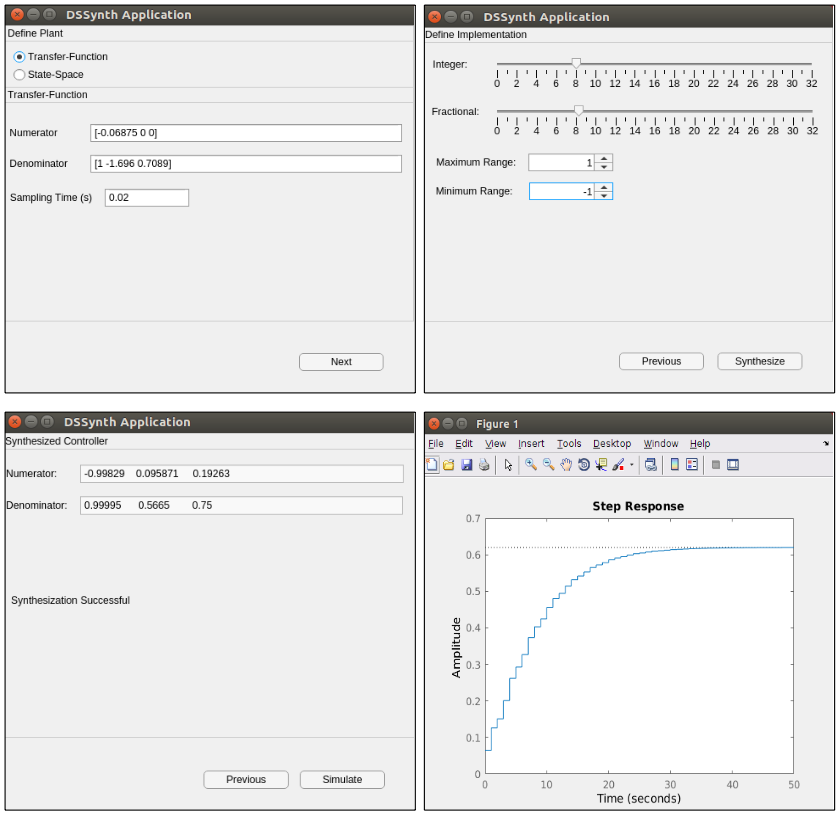
\includegraphics[width=0.5\textwidth]{screens_dssynth.png}
  \caption{GUI Application for Transfer-Function Synthesis.}
  \label{fig:gui-for-tf}
\end{figure}


%---------------------------------------------------
\subsection{Illustrative Example}
%---------------------------------------------------

To illustrate the \tool's usage, Fig.~\ref{toolbox-usage} shows the synthesis for a physical plant defined in Eq.(~\ref{equation_plant}) using the transfer-function representation, where ``num'' and ``den'' represent the numerator $A(z)$ and denominator $B(z)$, respectively.
%
\begin{equation}
\label{equation_plant}
H(z)=\frac{B(z)}{A(z)}=\frac{-0.06875z^{2}}{z^2-1.696z+0.7089},
\end{equation}
%
\begin{figure}[ht]
\scriptsize
\begin{lstlisting}[xleftmargin=.025\textwidth,xrightmargin=.025\textwidth, frame=single,]
>> num = [-0.06875 0 0];
>> den = [1.0000 -1.696 0.7089];
>> system = tf(num,den,0.002);
>> y = synthesize(system,8,8,1,-1);
>> SYNTHESIS SUCCESSFUL
>> y = (-0.9983z^2 + 0.09587z + 0.1926)/(z^2+0.5665+0.75);
\end{lstlisting}
\vspace{-0.2cm}
\caption{Synthesis of a Digital Controller for the physical plant defined in Eq.(~\ref{equation_plant}) in MATLAB, with a fixed-point format  $\left\langle 8,8\right\rangle$.}
\label{toolbox-usage}
\end{figure}
%
In the Fig.~\ref{toolbox-usage}, the value returned in $y$ represents the digital controller synthesized and stable. In order to validate and reproduce the stability in the digital system composed by the physical plant defined in Eq.(~\ref{equation_plant}) and the digital controller represented by $y$, the user can invoke the step response using the command \texttt{dstep}, and then observe that the graph plotted shows a stable digital system, as can be seen in Fig.~\ref{step-response}.
%
\begin{figure}[ht]
  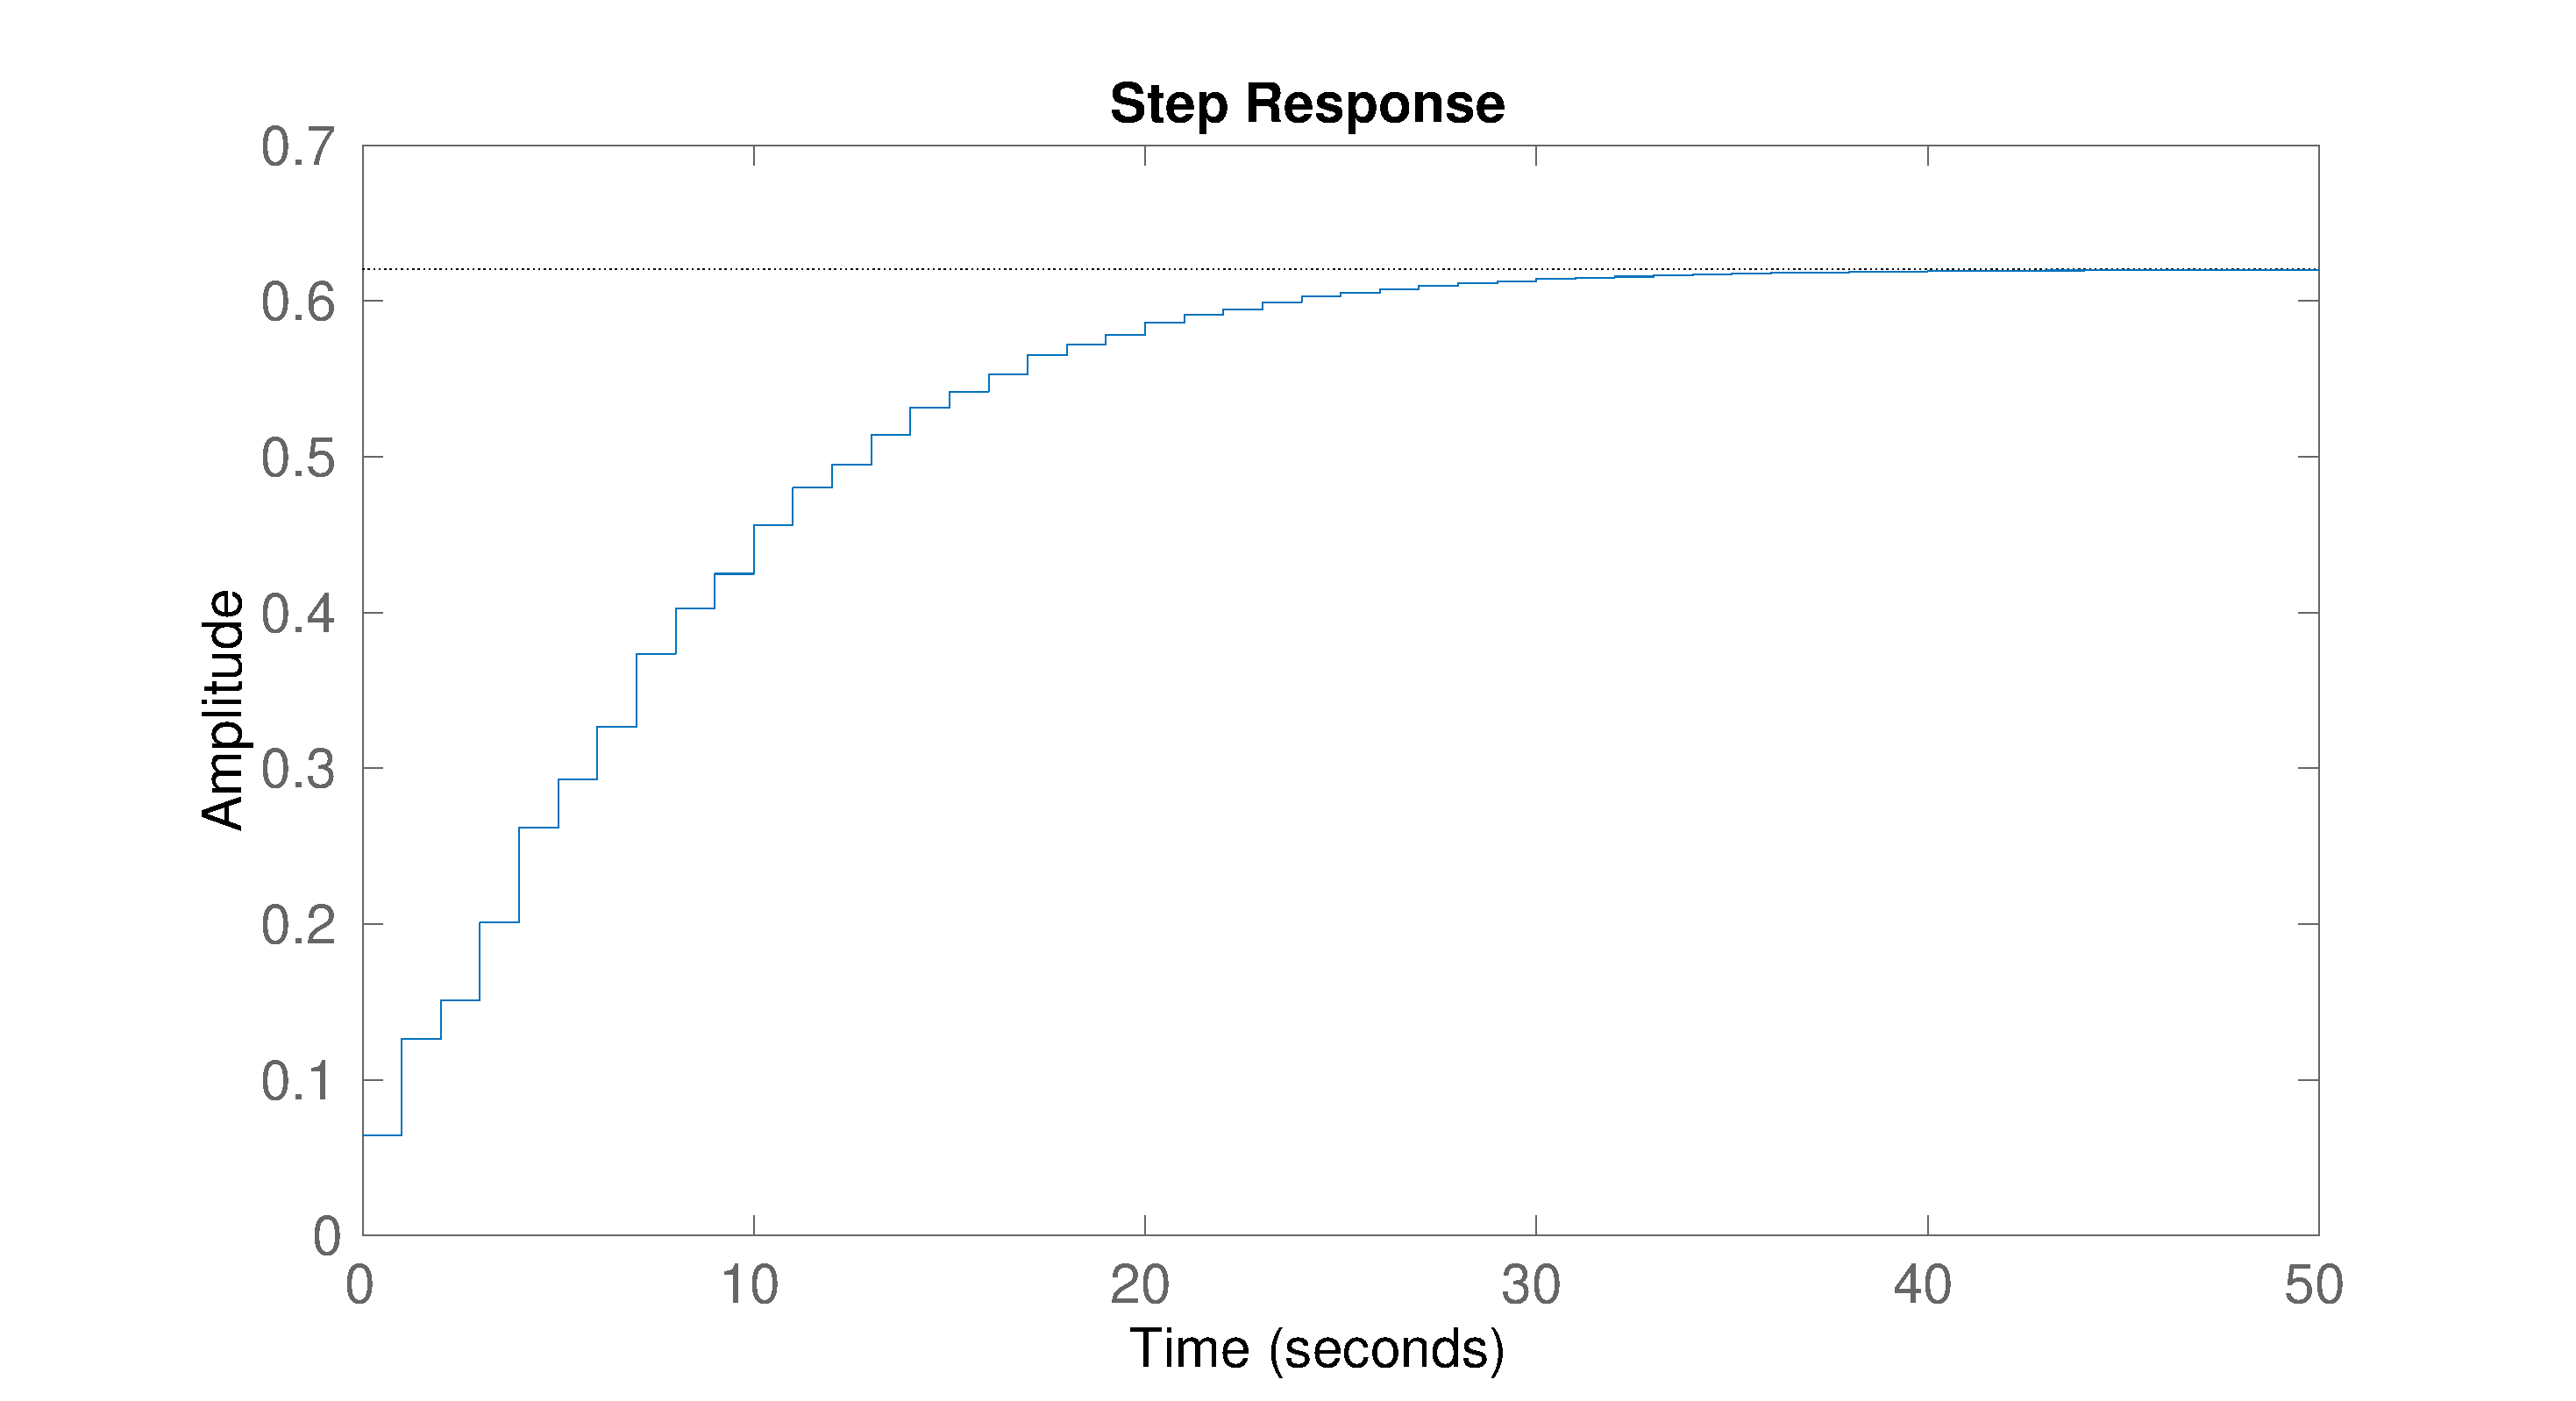
\includegraphics[width=0.5\textwidth]{step-response.eps}
  \caption{Step response for the Eq.~\eqref{equation_plant} describing a stable system.}
  \label{step-response}
\end{figure}


\section{Conclusions}

\tool is able to synthesize dynamic physical plants designed in MATLAB, through transfer-function and state-space representations based on Counter-Example Guided Inductive Synthesis (CEGIS)~\cite{DBLP:conf/asplos/Solar-LezamaTBSS06}.

Given the current literature in formal synthesis, there is no other MATLAB toolbox for synthesize stable digital systems, while taking into account implementation aspects (fixed-point arithmetic). 

As future work, \tool will perform synthesis to generate stable digital controllers and be combined with DSVerifier Toolbox~\cite{issta2017} to verify the stability of the digital controller synthesized, and also, with DSValidator Toolbox~\cite{dsvalidator}, in order to reproduce and validate the stability property.  


\bibliographystyle{ACM-Reference-Format}
\bibliography{references} 

\end{document}
